%%==============================================================================
%% 武汉理工大学学位论文 —— 主文件【2024 版·学术学位 / 专业硕士】
%%
%% 学位类型用文档类选项切换：
%%   [doctor]               博士（学术学位）
%%   [master]               硕士（学术学位，默认）
%%   [master,professional]  专业硕士（2024 版）
%%   再可叠加 [anonymous] 盲审、[fontset=mac] 切系统字体、[twoside] 双面
%%
%% 编译：latexmk -xelatex main-2024.tex   或   make V=2024
%%   手动：xelatex → bibtex → xelatex → xelatex
%%==============================================================================
\documentclass[doctor]{whut-thesis}

%%==============================================================================
%% 论文元信息：请在此处填写自己的题目、作者、导师等信息
%%==============================================================================

% ---- 题名与作者 ----
\ctitle{毕业论文中文题目}
\etitle{English Title of the Thesis}
\cauthor{张三}
\eauthor{Zhang San}
\studentid{1049721900001}

% ---- 学科信息 ----
\discipline{工学}                       % 学科门类：工学 / 理学 / 艺术学 ……
\cmajor{某一级学科}                      % 学科专业（中文）
\emajor{Discipline Name}                % 学科专业（英文）
\cdepartment{某某学院}                   % 培养单位 / 学院
\cfield{某研究方向}                      % 研究方向

% ---- 导师信息 ----
\cadvisor{李四}
\advisortitle{教授}
\advisordegree{博士}
\advisordept{某某学院}
\advisorzip{430070}
% 副导师（如无可留空）
\csubadvisor{}
\subadvisortitle{}
\subadvisordegree{}
\subadvisordept{}
\subadvisorzip{}

% ---- 题名页其它字段 ----
\classification{}             % 分类号
\secretlevel{公开}            % 密级
\udc{}                        % UDC
\schoolcode{10497}            % 学校代码（武汉理工大学，默认 10497）
\chairman{王五}               % 答辩委员会主席
\reviewer{盲审}               % 评阅人
\committee{赵六 教授、钱七 教授、孙八 研究员}  % 答辩委员会委员（顿号分隔）
\submitdate{2026.03.16}       % 论文提交日期
\defenddate{2026.05.19}       % 论文答辩日期
\cdate{2026 年 5 月}          % 封面日期
        % 论文元信息

\begin{document}

%% ---------------- 前置 ----------------
\makecover
\maketitlepage
\makedeclaration

\frontmatter
%%==============================================================================
%% 中文摘要 / 英文摘要
%%==============================================================================

\begin{cabstract}
随着智能制造的快速发展，人机协作已成为现代工业生产的重要模式。然而，在动态、
非结构化的协作环境中，如何对人与机器人的任务进行实时、高效的规划，仍然是一个
具有挑战性的问题。本文以工业人机协作场景为研究对象，从任务建模、动态规划与
策略优化三个方面开展研究，主要工作如下：

（1）针对人机协作任务的不确定性，建立了基于马尔可夫决策过程的任务规划模型，
将人的行为意图作为环境状态的一部分进行建模，提高了任务分配的合理性。

（2）针对动态环境下的实时规划需求，提出了一种基于深度强化学习的动态任务规划
方法。通过设计兼顾效率与安全的奖励函数，使智能体能够在协作过程中自适应地调整
任务分配策略。

（3）搭建了人机协作实验平台，在多种工况下验证了所提方法的有效性。实验结果
表明，与传统方法相比，本文方法在任务完成时间和协作安全性方面均具有明显优势。

\ckeywords{人机协作；深度强化学习；动态任务规划；智能制造；马尔可夫决策过程}
\end{cabstract}

\begin{eabstract}
With the rapid development of intelligent manufacturing, human-robot collaboration
(HRC) has become an important paradigm in modern industrial production. However,
how to plan the tasks of humans and robots in real time and efficiently in a dynamic
and unstructured collaborative environment remains a challenging problem. This thesis
takes the industrial HRC scenario as the research object and carries out research from
three aspects: task modeling, dynamic planning, and policy optimization. The main
work is as follows:

(1) To address the uncertainty of HRC tasks, a task planning model based on the Markov
decision process is established, in which human behavioral intention is modeled as part
of the environment state, improving the rationality of task allocation.

(2) To meet the real-time planning requirements in dynamic environments, a dynamic
task planning method based on deep reinforcement learning is proposed. By designing a
reward function that balances efficiency and safety, the agent can adaptively adjust the
task allocation policy during collaboration.

(3) An HRC experimental platform is built, and the effectiveness of the proposed method
is verified under various working conditions. Experimental results show that, compared
with traditional methods, the proposed method has obvious advantages in task completion
time and collaboration safety.

\ekeywords{Human-Robot Collaboration; Deep Reinforcement Learning; Dynamic Task
Planning; Intelligent Manufacturing; Markov Decision Process}
\end{eabstract}

\tableofcontents

%% ---------------- 正文 ----------------
\mainmatter
%%==============================================================================
%% 第一章 绪论（示例占位内容，请替换）
%%==============================================================================
\chapter{绪论}\label{chap:intro}

\section{研究背景与意义}
本节为示例占位内容，用于演示正文排版。正文采用宋体小四号，行距为固定值约二十磅，
段落首行缩进两个字符。请将此处替换为研究背景与意义的实际论述。

正文中引用参考文献时，使用上标数字标注，例如已有研究\cite{ref-journal}对相关问题进行了
讨论，另有若干工作\cite{ref-book,ref-thesis}也有所涉及。请将本段替换为实际内容。

\section{国内外研究现状}

\subsection{某方面研究现状}
本小节为示例占位内容。请将此处替换为某一方面研究现状的综述，并在适当位置标注
参考文献\cite{ref-conf}。

\subsection{某方面研究现状}
本小节为示例占位内容。请将此处替换为另一方面研究现状的综述\cite{ref-en}。

\section{本文主要研究内容}
本文的章节安排如下：
\begin{enumerate}[label={（\arabic*）},leftmargin=*]
  \item 第二章介绍相关理论与研究方法；
  \item 第三章给出实验设计与结果分析；
  \item 第四章总结全文并展望后续工作。
\end{enumerate}

%%==============================================================================
%% 第 2 章 人机协作动态任务规划建模
%%==============================================================================
\chapter{人机协作动态任务规划建模}\label{chap:method}

\section{引言}
本章将人机协作任务规划问题形式化为马尔可夫决策过程，并给出状态、动作与奖励的
定义。

\section{马尔可夫决策过程建模}
将人机协作系统建模为五元组 $\mathcal{M}=(\mathcal{S},\mathcal{A},P,R,\gamma)$，
其中 $\mathcal{S}$ 为状态空间，$\mathcal{A}$ 为动作空间，$P$ 为状态转移概率，
$R$ 为奖励函数，$\gamma\in(0,1]$ 为折扣因子。智能体的目标是最大化累积折扣
回报，如式~\eqref{eq:return} 所示：
\begin{equation}\label{eq:return}
  G_t = \sum_{k=0}^{\infty} \gamma^{k} R_{t+k+1}.
\end{equation}

最优策略 $\pi^{*}$ 满足贝尔曼最优方程~\eqref{eq:bellman}：
\begin{equation}\label{eq:bellman}
  Q^{*}(s,a) = \mathbb{E}\!\left[ R_{t+1}
    + \gamma \max_{a'} Q^{*}(s',a') \,\middle|\, s,a \right].
\end{equation}

\begin{definition}[协作安全裕度]\label{def:safety}
设人与机器人末端的最小距离为 $d_{\min}$，安全阈值为 $d_{s}$，则协作安全裕度
定义为 $\eta = (d_{\min}-d_{s})/d_{s}$。
\end{definition}

\begin{theorem}\label{thm:converge}
在折扣因子 $\gamma<1$ 且奖励有界的条件下，值迭代算法收敛到唯一最优值函数。
\end{theorem}
\begin{proof}
由 Bellman 最优算子的 $\gamma$-压缩性质，结合 Banach 不动点定理即可证得，
此处从略。
\end{proof}

\section{系统框架}
本文提出的动态任务规划系统框架如图~\ref{fig:framework} 所示。系统由感知模块、
决策模块与执行模块组成。

\begin{figure}[htbp]
  \centering
  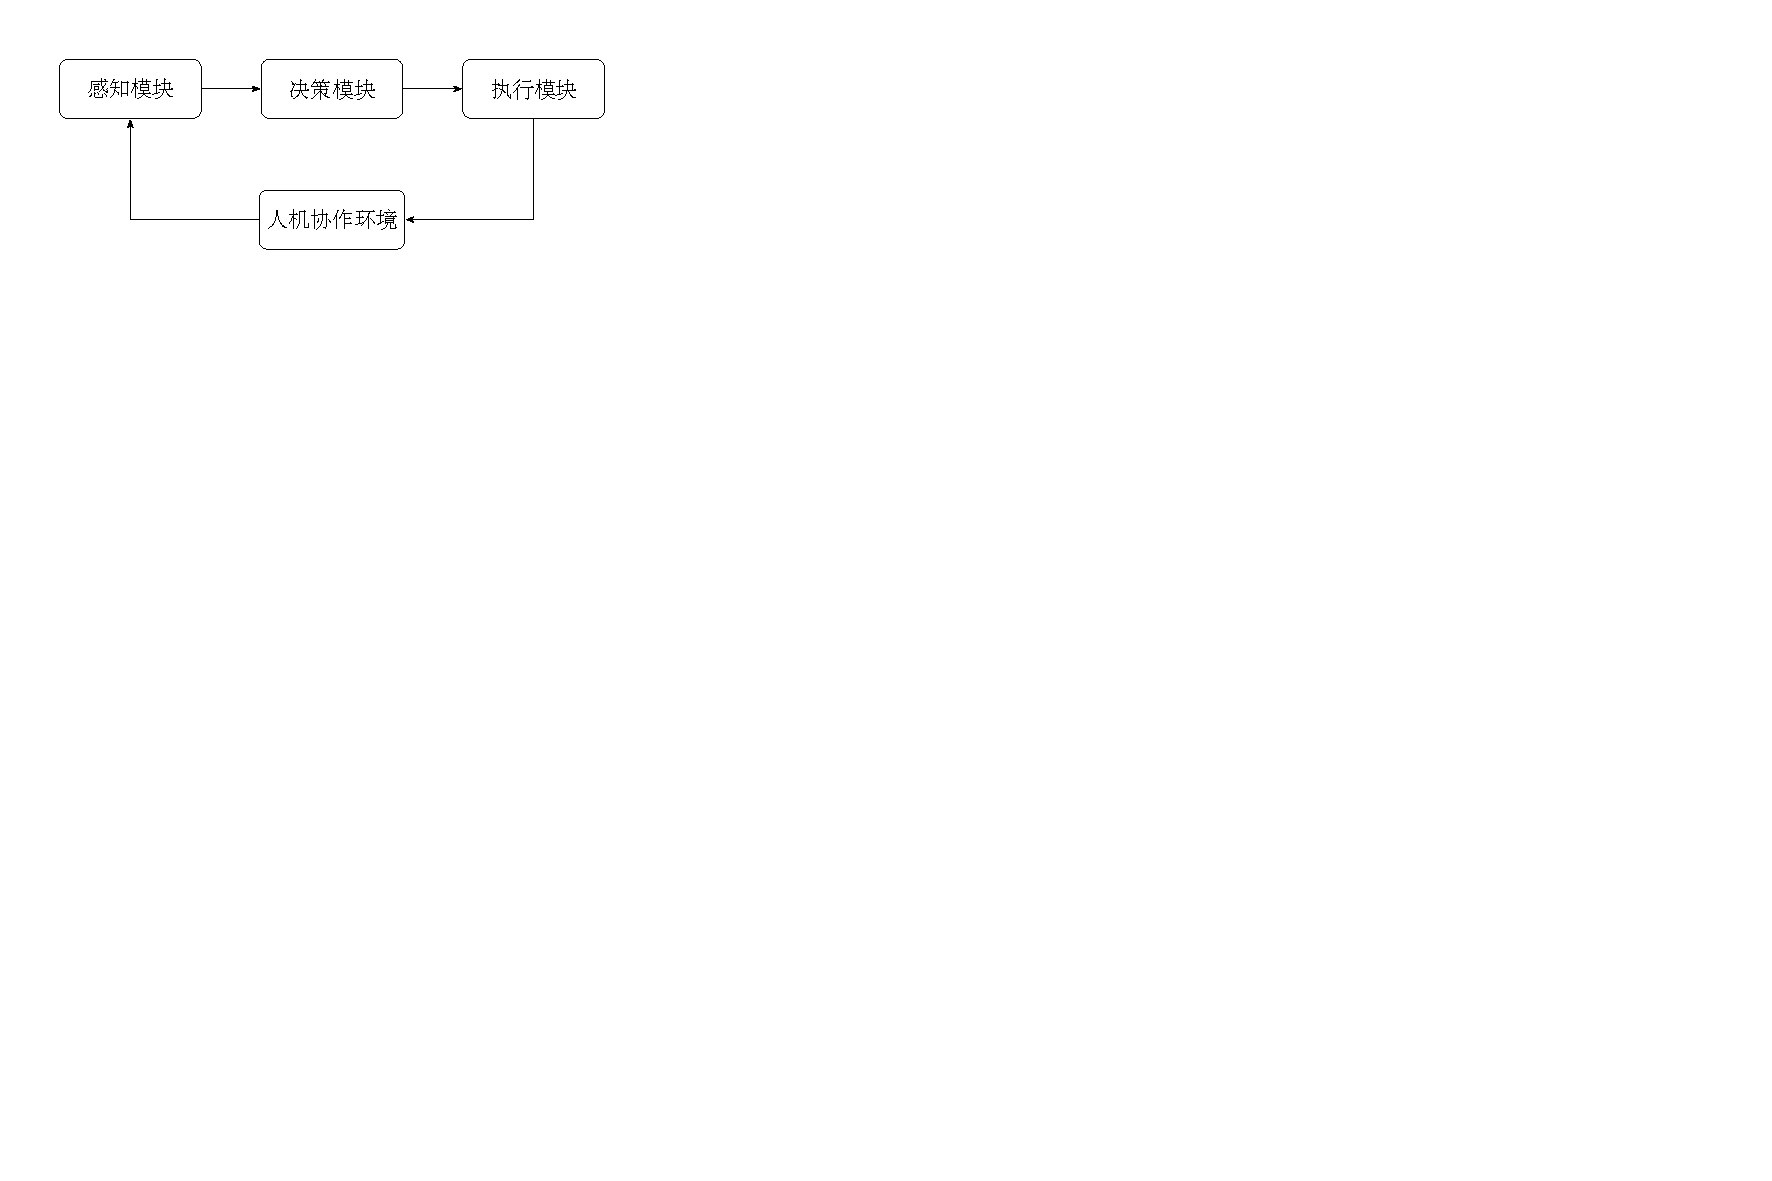
\includegraphics[width=0.7\textwidth]{figures/example-figure.pdf}
  \caption{人机协作动态任务规划系统框架}
  \label{fig:framework}
\end{figure}

\section{本章小结}
本章建立了人机协作动态任务规划的马尔可夫决策过程模型，给出了协作安全裕度的
定义，并证明了值迭代算法的收敛性，为后续算法设计奠定了基础。

%%==============================================================================
%% 第 3 章 实验与结果分析
%%==============================================================================
\chapter{实验与结果分析}\label{chap:experiment}

\section{实验设置}
实验在搭建的人机协作平台上进行，对比了本文方法与两种基线方法的性能。实验
主要参数如表~\ref{tab:params} 所示。

\begin{table}[htbp]
  \centering
  \caption{实验主要参数设置}
  \label{tab:params}
  \begin{tabular}{lcc}
    \toprule
    参数 & 符号 & 取值 \\
    \midrule
    学习率      & $\alpha$  & $3\times10^{-4}$ \\
    折扣因子    & $\gamma$  & $0.99$ \\
    经验回放容量 & $N$       & $10^{5}$ \\
    安全阈值    & $d_{s}$   & $0.2$ m \\
    \bottomrule
  \end{tabular}
\end{table}

\section{结果分析}
不同方法的任务完成时间对比如表~\ref{tab:results} 所示。可以看出，本文方法在
任务完成时间上较基线方法有明显降低。

\begin{table}[htbp]
  \centering
  \caption{不同方法性能对比}
  \label{tab:results}
  \begin{tabular}{lccc}
    \toprule
    \multirow{2}{*}{方法} & 完成时间 & 碰撞次数 & 成功率 \\
                          & (s)      & (次)     & (\%)   \\
    \midrule
    基线 A      & $42.3$ & $5$ & $86.0$ \\
    基线 B      & $38.7$ & $3$ & $91.5$ \\
    本文方法    & $\mathbf{31.5}$ & $\mathbf{0}$ & $\mathbf{98.2}$ \\
    \bottomrule
  \end{tabular}
\end{table}

由定理~\ref{thm:converge} 可知，所提算法在训练过程中能够稳定收敛，这与图中
所示的实验现象一致。

\section{本章小结}
本章在人机协作平台上验证了所提方法的有效性，实验结果表明本文方法在效率与
安全性方面均优于对比方法。

%%==============================================================================
%% 第四章 总结与展望（示例占位内容，请替换）
%%==============================================================================
\chapter{总结与展望}\label{chap:conclusion}

\section{全文总结}
本节为示例占位内容。请概括全文的主要工作，例如：
\begin{enumerate}[label={（\arabic*）},leftmargin=*]
  \item 完成了第一项主要工作；
  \item 完成了第二项主要工作；
  \item 完成了第三项主要工作。
\end{enumerate}

\section{研究展望}
本节为示例占位内容。请说明研究的不足之处与未来可进一步开展的工作方向。


%% ---------------- 后置（官方顺序：致谢→参考文献→科研成果目录→附录）----------------
%%==============================================================================
%% 致谢（研究生；示例占位，请替换为本人致谢）
%%==============================================================================
\begin{acknowledgement}
本部分为致谢示例占位文字。值此论文完成之际，谨向在学习与研究过程中给予指导和帮助的
师长、同学与亲友表示衷心的感谢。请将此处替换为本人的致谢内容。

本部分为致谢示例占位文字。请将此处替换为对导师、实验室同学以及家人的感谢。
\end{acknowledgement}
      % 致谢

\bibliography{ref}               % 参考文献（GB/T 7714-2015）

%%==============================================================================
%% 攻读学位期间发表的论文及科研成果
%%==============================================================================
\begin{publications}
  \item 张三, 李四. 基于深度强化学习的人机协作动态任务规划方法[J].
        自动化学报, 2026, 52(3): 1--12.
  \item Zhang San, Li Si. Dynamic task planning for human-robot collaboration
        via deep reinforcement learning[C]. Proceedings of the IEEE International
        Conference on Robotics and Automation (ICRA), 2025: 1234--1240.
  \item 张三, 李四, 王五. 一种人机协作任务分配方法及装置:
        中国, ZL2025XXXXXXXX.X[P]. 2026.
\end{publications}
         % 科研成果目录

%%==============================================================================
%% 附录（论文主体的补充项目，如长公式推导、程序代码、调查问卷、补充数据等）
%%==============================================================================
\begin{appendixpart}
\section*{附录 A\quad 主要符号对照表}
\addcontentsline{toc}{section}{附录 A\quad 主要符号对照表}

\begin{center}
\begin{tabular}{cl}
  \toprule
  符号 & 含义 \\
  \midrule
  $\gamma$    & 折扣因子 \\
  $\pi^{*}$   & 最优策略 \\
  $d_{\min}$  & 人机最小距离 \\
  \bottomrule
\end{tabular}
\end{center}

\section*{附录 B\quad 核心算法伪代码}
\addcontentsline{toc}{section}{附录 B\quad 核心算法伪代码}

附录可放置不便置于正文的补充材料，例如较长的推导、源代码、问卷、补充图表等。
\end{appendixpart}
             % 附录（如无可删去此行）

\end{document}
